% select subfiles base file
\documentclass[TGAI_Laborbericht.tex]{subfiles}
\begin{document}


\chapter{Versuch 1}
\label{chap:VERSUCH_1}


\section{Fragestellung, Messprinzip, Aufbau, Messmittel}
\label{chap:VERSUCH_1_FRAGESTELLUNG}

Im ersten Teil war gefordert, dass wir mithilfe eines Mikrofon einen Mundharmonika Ton per Oszilloskop einlesen und anschließend die Fouriertransformierte des Signals grafisch darstellen.

\subsection{Messmittel}
Als Messmittel dient ein 250g schweres Dynamisches Mikrofon mit einer Tauchspule (engl. moving coil). Es ist Uni-direktional und reagiert auf Frequenzen im Bereich von 70Hz bis 13 KHz und hat eine Sensitivität von -54dB $\pm$ 3dB. Die Ausgangs impendanz beträgt 500$\Omega \pm$30\%.

\subsection{Messprinzip}
Das Tauchspulenmikrofon (auch Tauchspulmikrofon) ist ein elektroakustischer Wandler, der nach dem elektroinduktiven Prinzip des dynamischen Mikrofons arbeitet. Es ist sowohl die Bauform des Druckgradientenmikrofons als auch die des Druckmikrofons üblich.

Der Begriff Tauchspulenmikrofon bezieht sich auf die technische Anordnung der Bauelemente des Wandlers: Bei dem Tauchspulenmikrofon ist die Membran fest mit einer Magnet-Spule verbunden, die durch die Membranbewegung in ein statisches dauermagnetisches Feld „eintaucht“. Siehe auch: Tauchspule. Die relative Bewegung von Spule und Magnetfeld erzeugt per Induktion die Signalspannung. Diese ist proportional zur Membrangeschwindigkeit.

Tauchspulenmikrofone benötigen keine nachträgliche Impedanzanpassung und auch keine Symmetrierung; beides kann allein durch die Dimensionierung und Verschaltung der Spule erreicht werden.

Prinzipielle Nachteile: Die Schallwelle muss die Masse der Membran mit der Spule bewegen und elektrische Arbeit leisten. Tauchspulenmikrofone haben daher eine geringe Empfindlichkeit und zeigen eine Trägheit im Einschwingverhalten, wodurch feinste Details nicht erfasst werden, was jedoch erwünscht sein kann: Sie liefern ein „erdiges“, kräftiges Klangbild, hochwertige Modelle werden daher durchaus auch bei Studioaufnahmen verwendet. Tauchspulenmikrofone haben ein nicht so hohes Übertragungsspektrum wie Kondensatormikrofone und sind aufgrund ihrer geringen Empfindlichkeit für Fernaufnahmen ungeeignet. Die relativ hohe Masse des Membransystems lässt sie zudem empfindlich auf Körperschall, etwa Hantierungsgeräusche, reagieren; um solche Störungen zu verringern, ist bei hochwertigen Tauchspulenmikrofonen die gesamte technische Einheit (die Mikrofonkapsel) im Mikrofongehäuse schwingfähig gelagert.

Die Vorteile dieses Mikrofontyps zeigen sich darin, dass sie in der Regel gegenüber mechanischen Belastungen recht robust sind und hohe Schalldrücke vertragen. Auch benötigen sie keine Spannungsversorgung, was im mobilen Betrieb von Vorteil sein kann. Die einfache Bauart erlaubt preisgünstige Fertigung und macht diesen Mikrofontyp nahezu unverwüstlich.


\subsection{Aufbau}
Das Mikrofon ist über ein Kabel mit dem Oszilloskop verbunden. Als Tonerzeuger benutzen wir eine Handelsübliche Mundharmonika, bei welcher wir Alle Löcher bis auf eines zugeklebt haben. Dies tun wir um zu verhindern, dass mehrere Töne gleichzeitig gespielt werden.

\section{Messwerte}
\label{chap:VERSUCH_1_MESSWERTE}
Während wir mit der Mundharmonika einen Ton in das Mikrofon spielen, zeichnen wir die Messwerte mithilfe des Oszilloskopes auf, indem wir den Knopf "Single Seq" drücken. Diese Momentaufnahme übertragen wir nun mithilfe eines Pythonskriptes an den PC. Hierzu importieren wir das Modul TekTDS2000. Dieses stellt uns die Funktion getData() zur verfügung, welches uns ein Array aus Messdaten übergibt.

\begin{figure}[H]
	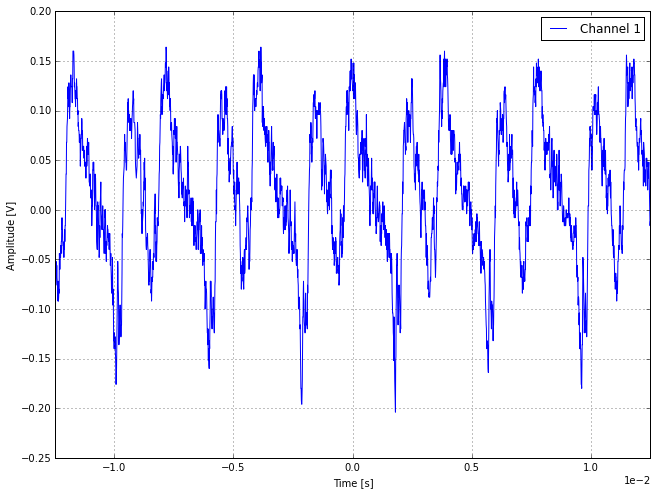
\includegraphics[width=0.7\textwidth]{media/V1.png}
	\label{fig:Ton}
	\caption{Ton}
\end{figure}

\section{Auswertung}
\label{chap:VERSUCH_1_AUSWERTUNG}
Auf die eingelesenen Werte wenden wir nun die Fouriertransformation mithilfe der numpy Funktion fft.fft() an. Hieraus berechnen wir nun das Amplitutenspektrum, nun haben wir noch das Problem, dass die Frequenzachse in Anzahl Schwingungen innerhalb der gesamten Signaldauer vorliegt und wir diese noch in Herz umrechnen müssen. Hierzu benutzen wir die Formel \[f=\frac{n}{M\cdot \Delta t}\] Nun können wir die Grundfrequenz bestimmen (252 Hz) und die dazugehörige Amplitude (0,026).



\section{Interpretation}
\label{chap:VERSUCH_1_INTERPRETATION}
Durch die Fouriertransformation waren wir in der Lage die Grundfrequenz und somit die Tonhöhe zu bestimmen. Desweiteren können wir dessen Amplitude berechnen und somit die Lautstärke.
\end{document}

\begin{figure}[H]
	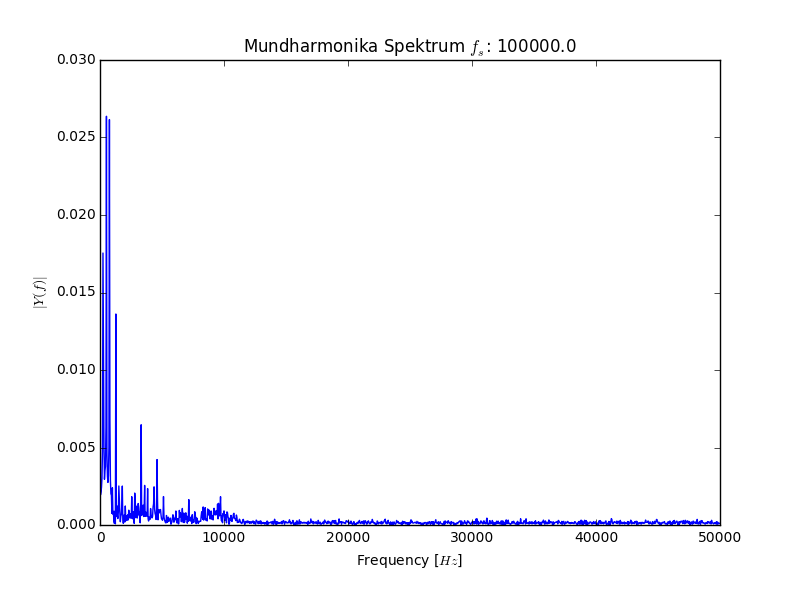
\includegraphics[width=0.7\textwidth]{media/v1_fft.png}
	\label{fig:fouriertransformierte}
	\caption{fouriertransformierte}
\end{figure}